\chapter{Automatisation du processus d'investigation}
\label{Automatisation du processus d'investigation}
\thispagestyle{fancy}
Lorsqu'une \emph{error name} est révélée durant le Filtering test, de nombreuses données sont enregistrées dans un fichier journal (que l'on retrouve plus souvent sous le terme anglais de fichier "log".) Une analyse poussée de ces informations permet de déterminer la \emph{root cause} liée à l'\emph{error name} (partie \ref{Introduction:Expression du besoin:Hiérarchisation des erreurs}). Afin d'automatiser ce processus d'analyse, on s'appuie sur l'utilisation d'algorithmes d'apprentissage automatique. 

\section{Architecture High Level du système proposé}
\label{Automatisation du processus d'investigation: Achitecture High Level du système proposé}
L'architecture haut niveau de la solution que l'on propose est composée de deux couches: une couche \emph{root cause} et une couche \emph{error name}.
\begin{description}
	\item [Couche root cause] La couche \emph{root cause} permet de détecter la présence d'une \emph{root cause} dans le fichier log que l'on analyse. Il s'agit d'un algorithme d'apprentissage automatique entraîné à effectuer cette tâche.
	\item [Couche error name] La couche \emph{error name} est constituée d'un ensemble de couches \emph{root cause} de telle manière que lorsqu'un fichier log est mis en entrée du système, l'ensemble des couches \emph{root cause} sont activées. Ainsi, le système recherche la présence de chaque \emph{root cause} connue dans l'exemple étudié. On dit que les \emph{root causes} sont liées à l'\emph{error name}. On obtient en sortie de la couche \emph{error name} le nom de la \emph{root cause} ayant la plus forte probabilité d'avoir été reconnue.
\end{description} 

\subsubsection{Exemple de mise en place  d'une couche error name et de ses couches root cause}
\label{Automatisation du processus d'investigation: Achitecture High Level du système proposé: Exemple de mise en place  d'une couche error name et de ses couches root cause}
Afin d'exposer de manière concrète le fonctionnement de l'architecture haut niveau de la solution proposée, on soumet un exemple de mise en place d'une architecture de détection et son utilisation. \\

\paragraph{Mise en place du système de détection d'une root cause}
On souhaite dans un premier temps mettre en place l'architecture permettant de détecter la cause (\emph{root cause}) ayant entrainé la chute du robot lors du Filtering test (\emph{error name}). Cette étape consiste à créer les couches \emph{root cause}, i.e. entrainer différents algorithmes d'apprentissage automatique à reconnaître la \emph{root cause} pour laquelle ils ont été créés (figure \ref{fig:Creation des couches root cause}). Afin d'entraîner ces couches, on utilise les données utiles à chaque \emph{root cause}, contenues dans le fichier log généré lors de la chute d'un robot durant le Filtering Test. Par exemple, dans le cas de la \emph{root cause} "frottement des freins de la hanche", on utilisera les données "valeurs du senseur de la hanche" et "valeurs de l'actuateur de la hanche". Ces deux éléments correspondent aux features de notre système d'apprentissage (c.f. partie \ref{Le Machine Learning: Généralités sur le Machine Learning: Définition et principe général:Lexique}). L'ensemble de ces couches \emph{root cause} sont liées une couche \emph{error name}, Ici la chute d'un robot.

\begin{figure}[h]
	\centering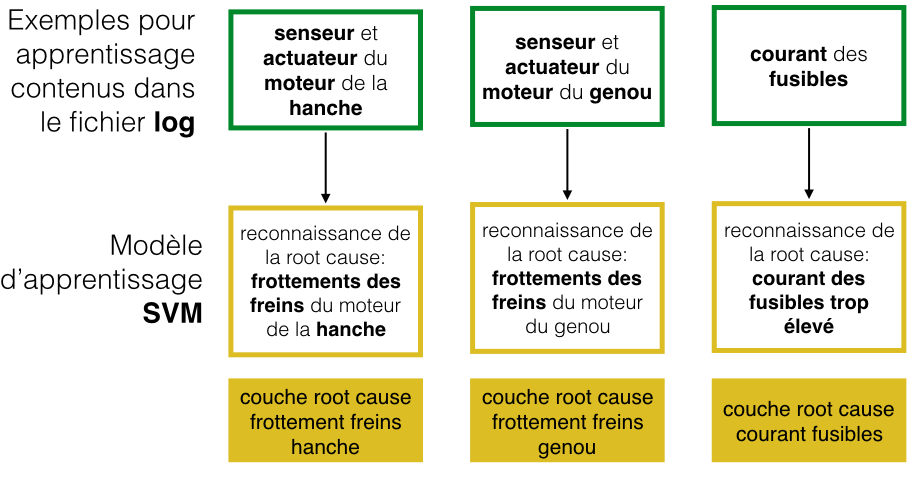
\includegraphics[height=7cm]{images/synoptique_root.png}
	\caption[Création des couches root cause]{Synoptique haut niveau de la création des couches \emph{root cause}. Les couches \emph{root cause} correspondent à des algorithmes d'apprentissage automatique que l'on entraîne à détecter la \emph{root cause} à laquelle ils sont associés. Par exemple, créer la couche \emph{root cause} "frottement du frein de la hanche" revient à entraîner un algorithme d'apprentissage de type SVM, à partir des valeurs senseurs et actuateurs de la hanche des fichiers logs.}
	\label{fig:Creation des couches root cause}
\end{figure}

\paragraph{Utilisation du système de détection d'une root cause}
Une fois nos différentes couches \emph{root cause} créées, on souhaite utiliser notre système pour détecter la cause ayant entrainé la chute d'un robot (c.f. figure \ref{fig:utilisation de la couche error name}). Pour cela, on place à l'entrée de notre couche \emph{error name} le fichier log que l'on souhaite analyser. Chaque couche \emph{root cause} extrait de ce fichier les features qui lui sont liées (e.g. la \emph{root cause} "frottement des freins de la hanche" est liée aux features senseurs et actuateurs de la hanche). L'algorithme SVM de chaque couche \emph{root cause} va alors émettre une décision quant à la présence ou non de leur \emph{root cause} dans le fichier log. Cette décision correspond à la probabilité que la \emph{ root cause} ait été détectée (en \%). La couche \emph{root cause} ayant la probabilité la plus élevée en sortie est considérée comme la \emph{root cause} ayant entrainé l'\emph{error name},  ici la chute du robot) 

\begin{figure}[h]
	\centering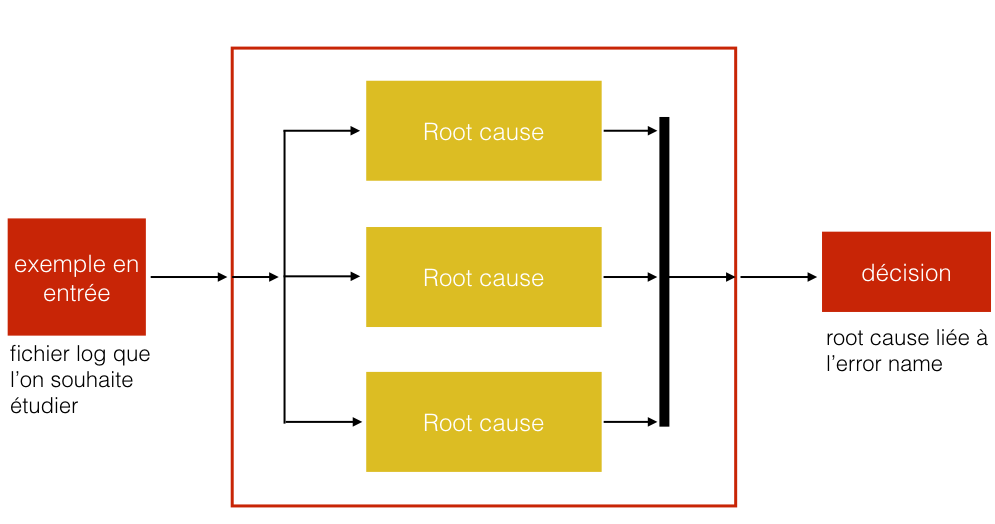
\includegraphics[width=15cm]{images/synoptique_error.png}
	\caption[Utilisation de la couche error name]{Synoptique haut niveau de l'utilisation de la couche \emph{error name}. La couche \emph{error name} contient plusieurs couches \emph{root cause} (on dit qu'elles sont liées). On met en entrée du système le fichier log que l'on souhaite analyser, puis chaque couche \emph{root cause} va détecter la présence de sa \emph{root cause}. On obtient en sortie de la couche \emph{error name} la \emph{root cause}  ayant eu la plus forte probabilité d'avoir été reconnue.}
	\label{fig:utilisation de la couche error name}
\end{figure}

Chaque couche \emph{root cause} peut être considérée comme un système d'apprentissage à part entière. Le schéma fonctionnel d'une \emph{root cause} (cf. figure 	\ref{fig:Synoptique d'une couche root cause}) reprend la même structure que celui du Machine Learning (c.f. \ref{fig:Schéma fonctionnel haut niveau du Machine Learning}). En effet, chaque \emph{root cause} est constituée d'une instance de l'algorithme SVM. Dans la suite de notre étude de l'architecture haut niveau, on s'intéressera plus particulièrement  au fonctionnement de la couche \emph{root cause}, celle-ci contenant l'ensemble du traitement et de l'analyse des données.

\begin{figure}[h]
	\centering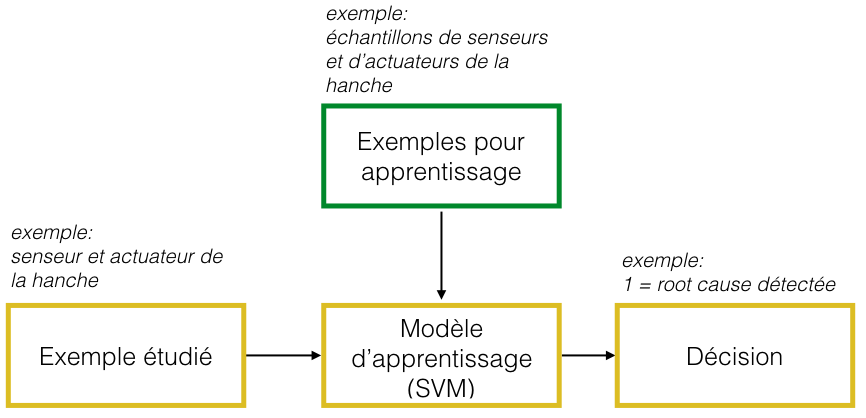
\includegraphics[height=7cm]{images/exemple_root.png}
	\caption[Synoptique d'une couche root cause]{Synoptique d'une couche \emph{root cause}. Il correspond à celui du Machine Learning car chaque couche \emph{root cause} est en réalité un algorithme d'apprentissage supervisé SVM que l'on entraine à détecter une \emph{root cause} particulière.}
	\label{fig:Synoptique d'une couche root cause}
\end{figure}

\subsection{Les exemples}
\label{Automatisation du processus d'investigation: Achitecture High Level du système proposé: Les exemples}
Les exemples sont les éléments permettant d'entraîner un algorithme d'apprentissage automatique (c.f. partie \ref{Le Machine Learning: Généralités sur le Machine Learning: Les données}). Dans le cadre de la résolution de notre problématique, ils correspondent aux données générées et enregistrées dans le fichier log lorsqu'une erreur (\emph{error name}) est détectée durant le Filtering Test.

\subsubsection{Structure du fichier log}
\label{Automatisation du processus d'investigation: Achitecture High Level du système proposé: Les exemples: Structure du fichier log}
Le fichier log renferme un ensemble de données enregistrées lors de la détection d'une erreur durant le Filtering Test. Elles correspondent aux "rythmes vitaux" du robot. Le fichier contient par exemple l'évolution temporelle des différents actuateurs et senseurs de Pepper, la température de différentes pièces mécaniques, etc. Dans le cadre de l'entraînement de l'algorithme du Machine Learning (SVM), chacune de ces constantes correspond à une feature  (c.f. partie  \ref{Le Machine Learning: Généralités sur le Machine Learning: Définition et principe général:Lexique}). Soit le tableau \ref {tab: Extrait du contenu d'un fichier log}, un extrait du contenu d'un fichier log:

\begin{equation}
\begin{blockarray}{ccccccc}
\begin{block}{c[cccccc]}
features & X_1 & X_2 & X_3 & X_4 &  X_5 & X_6 \\
t_0 & -0,404 & 0,64 & -0,023 & -0,04 & -0,008 & -0,007 \\
t_1 & -0,404 & 0,64 & -0,029 & -0,038 & -0,006 & -0,006 \\
t_3 & -0,404 & 0,576 & -0,029 & -0,033 & -0,008 & -0,012 \\
t_4 & -0,402 & 0,544 & -0,029 & -0,027 & -0,012 & -0,022 \\
t_5 & -0,401 & 0,448 & -0,029 & -0,027 & -0,015 & -0,029 \\
t_6 & -0,401 & 0,448 & -0,023 & -0,029 & -0,017 & -0,031 \\
t_7 & -0,408 & 0,096 & -0,021 & -0,031 & -0,015 & -0,032 \\
t_8 & -0,444 & 0,096 & -0,021 & -0,032 & -0,015 & 0,035 \\
t_9 & -0,486 & 0,096 & -0,021 & -0,033 & -0,017 & -0,039 \\
t_{10} & -0,523 & 0,128 & -0,021 & -0,033 & -0,018 & -0,043 \\
t_n & ... & ... & ... & ... & ... & ... \\
\end{block}
\end{blockarray}
\label {tab: Extrait du contenu d'un fichier log}
\end{equation}

Avec :
\begin{itemize}
	\item $X_1$ = HeadPitchPositionActuatorValue
	\item $X_2$ = HeadPitchElectricCurrentSensorValue
	\item $X_3$ = ipPitchPositionSensorValue
	\item $X_4$ = HipPitchPositionActuatorValue
	\item $X_5$ = KneePitchPositionSensorValue
	\item $ X_6$ = KneePitchPositionActuatorValue
\end{itemize}

Le fichier log, représenté par le tableau \ref {tab: Extrait du contenu d'un fichier log}, correspond à un exemple de la base de données qui sert à entrainer chacun de nos algorithmes. \\ 
A chaque colonne du tableau correspond une feature. Chacune des lignes est la valeur des features à un instant t (une ligne ne correspond pas à un exemple !). 

\subsubsection{Structure de la base de données d'exemples}
\label{Automatisation du processus d'investigation: Achitecture High Level du système proposé: Les exemples: Structure de la base de données d'exemples}
La base de donnée est composée de plusieurs exemples qui correspondent à des fichiers logs. Par exemple, dans le cadre de la construction de couche \emph{error name} de la chute d'un robot, la base de donnée sera constituée de fichiers logs générés par plusieurs cas de chutes sur différents robots. On peut représenter la structure des données de la base de données par le tableau \ref {tab: Structure de la base de données d'exemples pour l'entrainement du SVM}

\begin{equation}
\begin{blockarray}{ccccccc}
\begin{block}{c[cccccc]}
features & X_1 & X_2 & X_3 & X_4 &  X_5 & X_6 \\
exemple_0 & log_0 [X_1] & log_0 [X_2] & log_0 [X_3]& log_0 [X_4] & log_0 [X_5] & log_0 [X_6]  \\
exemple_1 & log_1 [X_1] & log_1 [X_2] & log_1 [X_3]& log_1 [X_4] & log_1 [X_5] & log_1 [X_6]  \\
exemple_2 & log_2 [X_1] & log_2 [X_2] & log_2 [X_3]& log_2 [X_4] & log_2 [X_5] & log_2 [X_6]  \\
exemple_3 & log_3 [X_1] & log_3 [X_2] & log_3 [X_3]& log_3 [X_4] & log_3 [X_5] & log_3 [X_6]  \\
exemple_4 & log_4 [X_1] & log_4 [X_2] & log_4 [X_3]& log_4 [X_4] & log_4 [X_5] & log_4 [X_6]  \\
exemple_4 & log_4 [X_1] & log_n [X_2] & log_n [X_3]& log_n [X_4] & log_n [X_5] & log_n [X_6]  \\
\end{block}
\end{blockarray}
\label {tab: Structure de la base de données d'exemples pour l'entrainement du SVM}
\end{equation}

Tout comme la structure d'un fichier log (\ref{Automatisation du processus d'investigation: Achitecture High Level du système proposé: Les exemples: Structure du fichier log}), chaque colonne correspond à une feature. Chaque ligne de ce tableau représente un exemple et correspond à un fichier log. Cela signifie que chaque ligne du tableau correspond au contenu d'un fichier log, présenté dans le tableau \ref {tab: Extrait du contenu d'un fichier log}.

\subsubsection{Construction d'une couche root cause à partir de la base de données d'exemples}
\label{Automatisation du processus d'investigation: Achitecture High Level du système proposé: Les exemples: Construction d'une couche root cause à partir de la base de données d'exemples}
Lorsque l'on veut construire une nouvelle couche \emph{root cause}, i.e. entraîner un nouvel algorithme d'apprentissage, pour détecter la présence d'une \emph{root cause} particulière dans un fichier log, on sélectionne uniquement les features de la base de données d'exemples liées à celle-ci. Par exemple, si on veut créer une nouvelle couche root cause "frottement des freins de la hanche" (lié à l'error name chute du robot), on n'utilisera que les features "HipPitchPositionSensorValue" et "HipPitchPositionActuatorValue" de notre base de données.

\subsubsection{Représentation des exemples et des classes}
\label{Automatisation du processus d'investigation: Achitecture High Level du système proposé: Les exemples: Représentation des exemples et des classes}
Pour construire chaque couche \emph{root cause}; on entraine l'algorithme de l'apprentissage automatique. Pour cela, on a besoin d'exemples labellisés positifs (dans notre cas, le terme positif signifie des exemples de motifs caractéristiques de la \emph{root cause}) et des exemples labellisés négatifs (des exemples qui ne correspondent pas au motif caractéristique de la \emph{root cause}). Ces deux groupes d'exemples forment alors des classes. Dans le cadre de la \emph{root cause} "frottement des freins de la hanche", on peut visualiser l'ensemble de ces exemples et ces classes dans un repère construit à partir des features "position du senseur de la hanche" (clé HipPitchPositionSensorValue) et "position de l'actuateur de la hanche" (clé HipPitchPositionActuatorValue) en figure 	\ref{fig:Représentation de la répartition des exemples et des classes en fonction des features}. Lors de la phase d'investigation, l'algorithme emet alors un choix entre ces deux classes: positive, i.e. présence de la \emph{root cause} dans le fichier log, négative, i.e. absence de la \emph{root cause} dans le fichier log. 

\begin{figure}[h]
	\centering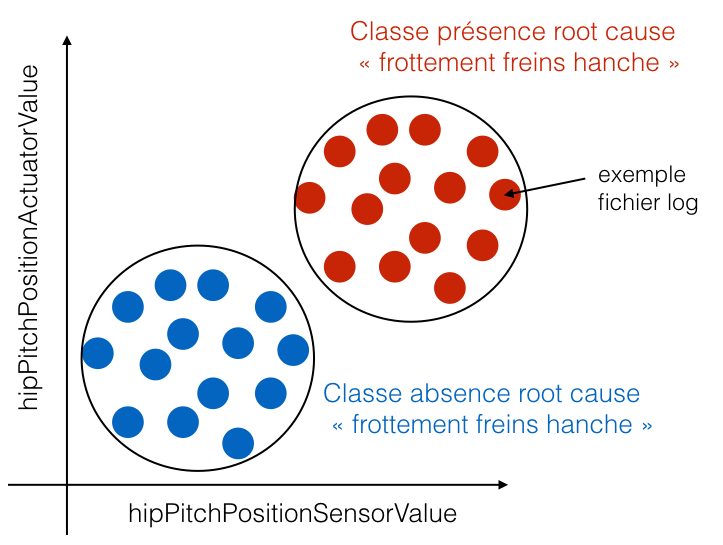
\includegraphics[width=9cm]{images/classes_log.png}
	\caption[Représentation de la répartition des exemples et des classes en fonction des features]{Représentation de la répartition des exemples et des classes en fonction des features. On observe que lorsque l'on visualise les exemples contenus dans nos fichiers logs en fonction des deux features HipPitchPositionSensorValue et HipPitchPositionActuatorValue, ces derniers se regroupent en deux zones homogène, qui forment nos classes. Une classe correspond aux exemples de \emph{root cause} "frottement des freins de la hanche", l'autre classe aux exemple qui ne correspondent pas à cette \emph{root cause}}.
	\label{fig:Représentation de la répartition des exemples et des classes en fonction des features}
\end{figure}

Cette représentation n'est pas fonctionnelle mais conceptuelle, i.e. qu'il ne s'agit pas d'une visualisation résultant d'un système fonctionnel de classification mais d'une idée haut niveau que l'on a de la sortie de notre système. 


\subsubsection{Parallèle avec l'exemple de la prévision saisonnière}
\label{Automatisation du processus d'investigation: Achitecture High Level du système proposé: Les exemples: Parallèle avec l'exemple de la prévision saisonnière}
Si on compare les échantillons utilisés dans l'exemple "prévisions saisonnières" (c.f. tableau \ref{exemples prévision saisonnière}) et ceux de notre solution (c.f. tableau \ref {tab: Structure de la base de données d'exemples pour l'entrainement du SVM}), on observe que dans les deux cas les données sont structurées en exemples et features. Cependant, dans la solution que l'on propose, les données de chaque exemple évoluent temporellement (e.g. la "HipPitchPositionSensorValue" de l'exemple 1 correspond à la colonne "HipPitchPositionSensorValue" du fichier $log_1$, qui a une évolution temporelle), alors que celles de la prévision saisonnière sont discrètes (e.g la température de l'exemple 1 est de -10\degres C, elle est discrète) \\
Or, on ne peut réaliser pas de l'apprentissage supervisé avec des données temporelles. Sous leurs formes actuelles, nos exemples ne peuvent donc pas servir à entrainer les algorithmes SVM de nos couches \emph{ root cause}.


\subsection{Le modèle d'apprentissage}
\label{Automatisation du processus d'investigation: Achitecture High Level du système proposé: Le modèle d'apprentissage}
Le modèle d'apprentissage utilisé est le Support Vector Machine (SVM) (cf. partie \ref{Le Machine Learning: Les différents algorithmes: SVM}).


\subsection{La décision}
\label{Automatisation du processus d'investigation: Achitecture High Level du système proposé: La décision}
Chaque couche \emph{root cause} délivre en sortie la probabilité que la \emph{root cause} à laquelle elle est rattachée soit présente dans le fichier log analysé (via le SVM).



\section{Détection d'une root cause}
\label{Automatisation du processus d'investigation: Détection d'une root cause}
On souhaite réaliser de la reconnaissance de motifs grâce à l'utilisation du SVM, pour détecter la présence d'une \emph{root cause} dans un fichier log. L'utilisation de cette méthode répond notamment au problème causé par l'évolution temporelle des exemples utilisés pour l'entraînement de l'algorithme (cf. partie \ref{Automatisation du processus d'investigation: Achitecture High Level du système proposé: Les exemples: Parallèle avec l'exemple de la prévision saisonnière}). On présente dans cette partie les différentes solutions envisagées et les raisons ayant amené à utiliser la reconnaissance de motifs. \\

Afin de simplifier le développement du système de reconnaissance de motifs, on admet dans un premier temps que chaque couche \emph{root cause} est un système d'apprentissage automatique, capable de détecter une \emph{root cause} en analysant \textbf{une seule} feature (e.g. BaseAccZ, HipPitchSensorValue, etc.) 

\subsection{Différentes approches étudiées}
\label{Automatisation du processus d'investigation: Reconnaissance de motifs: Différentes approches étudiées}
L'évolution temporelle des exemples utilisés pour l'entraînement de l'algorithme implique de prétraiter les données (c.f. partie \ref{Automatisation du processus d'investigation: Achitecture High Level du système proposé: Les exemples: Parallèle avec l'exemple de la prévision saisonnière}). Pour cela, différentes approches sont envisagées.

\subsubsection{Création de nouvelles features}
\label{Automatisation du processus d'investigation: Reconnaissance de motifs: Différentes approches étudiées: Création de nouvelles features}
On propose de créer de nouvelles features aux valeurs constantes. Elles sont des caractéristiques des features actuelles. Dans le cadre de cette étude, on les identifiera sous l'appellation de \emph{caractéristiques simplifiées}. Elles correspondent par exemple au calcul de la moyenne d'une feature, la valeur crête-à-crête, la valeur maximum, etc. On se sert ensuite de ces nouvelles \emph{caractéristiques simplifiées} pour réaliser l'entrainement de notre algorithme d'apprentissage automatique (c.f. exemple figure \ref{fig:Calcul de nouvelles features}).

\begin{figure}[h]
	\centering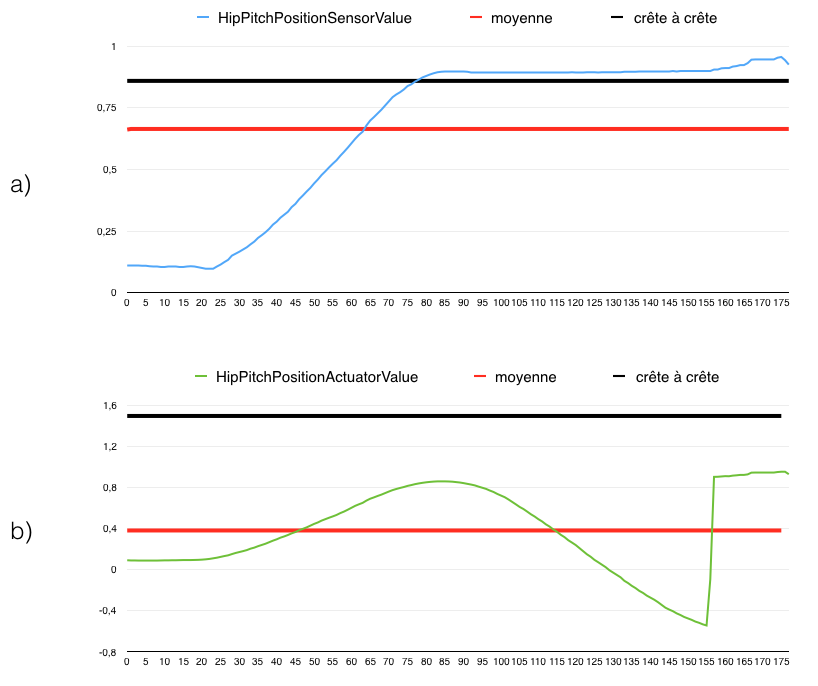
\includegraphics[width=12cm]{images/caracteristiques_simples_1.png}
	\caption[Calcul des caractéristiques simplifiées]{Calcul des \emph{caractéristiques simplifiées}. La figure représente l'évolution de la feature "accélération du robot selon l'axe $z$",  caractéristique de la chute d'un robot. La ligne rouge représente sa valeur moyenne. la ligne noire correspond à sa valeur crête-à-crête. On a ainsi réduit notre feature à deux valeurs constantes. On peut donc entraîner l'algorithme d'apprentissage automatique à partir de ces \emph{caractéristiques simplifiées}.}
	\label{fig:Calcul de nouvelles features}
\end{figure}

Le problème de cette approche est qu'elle réduit le nombre d'informations que contient une donnée à seulement quelques features (e.g. moyenne, valeur crête-à-crête). Comme le démontre la figure \ref{fig:Comparaison de deux caractéristiques}, cette diminution des informations peut entrainer des risques de confusion entre différentes features, i.e. deux features différentes peuvent avoir les mêmes caractéristiques. Or, si on souhaite utiliser cette approche dans l'architecture que l'on propose partie \ref{Automatisation du processus d'investigation: Achitecture High Level du système proposé}, le risque est que deux couches \emph{root cause} soient liées à des features dont les caractéristiques sont similaires. Dans ce cas, le système est incapable de déterminer quelle \emph{root cause} est responsable de l'apparition d'une \emph{error name}.

\begin{figure}[h]
	\centering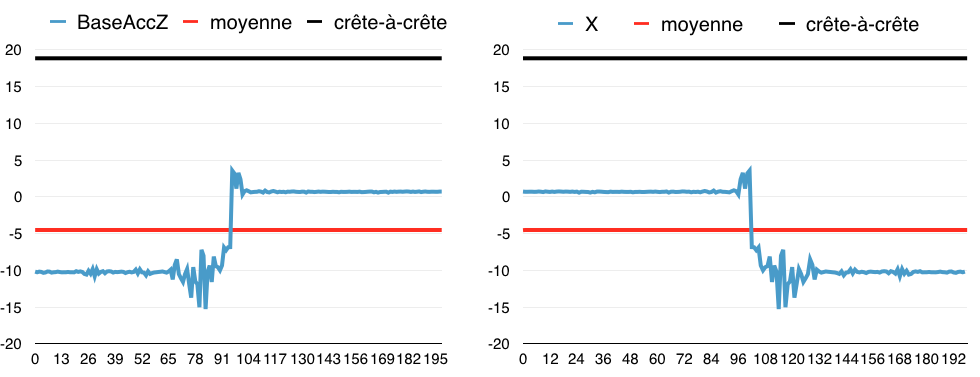
\includegraphics[width=15cm]{images/caracteristiques_simples_2.png}
	\caption[Comparaison de deux caractéristiques]{Calcul de nouvelles features. On retrouve sur la figure a) la valeur de l'accélération selon l'axe $z$ et ses caractéristiques simplifiées. Sur la figure b), on observe une autre feature et ses caractéristiques simplifiées. On remarque que, bien qu'il s'agisse de features différentes entres les figures a) et b), ces dernières possèdent les mêmes caractéristiques simplifiées.}
	\label{fig:Comparaison de deux caractéristiques}
\end{figure}

\subsubsection{Considérer chaque unité de temps comme une feature}
\label{Automatisation du processus d'investigation: Reconnaissance de motifs: Différentes approches étudiées: Considérer chaque unité de temps comme une feature}
On propose de considérer chaque unité de temps comme une feature. Le nombre d'entrées du système d'apprentissage automatique est donc égal au nombre d'échantillons contenus dans un exemple (cf. figure \ref{fig:Considérer chaque unité de temps comme une feature: exemple}). \\
De manière intuitive, entrainer le modèle revient à créer un patron représentatif de la feature lorsqu'elle est liée à la présence d'une \emph{root cause}. Une fois cette forme apprise, on la compare avec la feature que l'on souhaite analyser afin de savoir si la \emph{root cause} est présente ou non dans la feature.
\newline

\paragraph{Exemple} On souhaite créer une nouvelle couche \emph{root cause} (i.e. entraîner un algorithme d'apprentissage) capable de reconnaitre lorsqu'un robot chute. Dans le cadre de notre problématique ce système n'a pas de réelle utilité, on le propose ici car le problème est simple à comprendre. \\
Pour savoir si le robot chute ou non, on analyse l'évolution de la valeur de l'accélération selon l'axe $z$, fournie par l'accéléromètre de la base de Pepper (clé BaseAccZ). \\
D'après la figure \ref{fig:Formes caractéristiques de BaseAccZ en temps normal et en cas de chute}, on remarque que l'évolution de BaseAccZ enregistrée lors de la chute d'un robot diffère de l'évolution de BaseAccZ lorsque le robot ne chute pas. On va entraîner à l'algorithme à reconnaitre la forme caractéristique de l'évolution de l'accélération en $z$ lorsque le robot chute. Pour cela, on admet que chaque échantillon (chaque instant t) qui constitue la BaseAccZ devient une entrée (feature) pour l'entrainement de l'algorithme d'apprentissage (cf. figure \ref{fig:Créer un patron caractéristique de la chute du robot}). \\
On compare ensuite ce patron à la courbe de l'accélération en $z$ contenue dans le fichier log que l'on souhaite étudier. Si elle est globalement similaire au patron, on en déduit que le robot a chuté. Dans le cas contraire, on en déduit que le robot n'a pas chuté (cf. figure \ref{fig:Détection d'une chute à partir du patron de BaseAccZ}).

\begin{figure}[h]
	\centering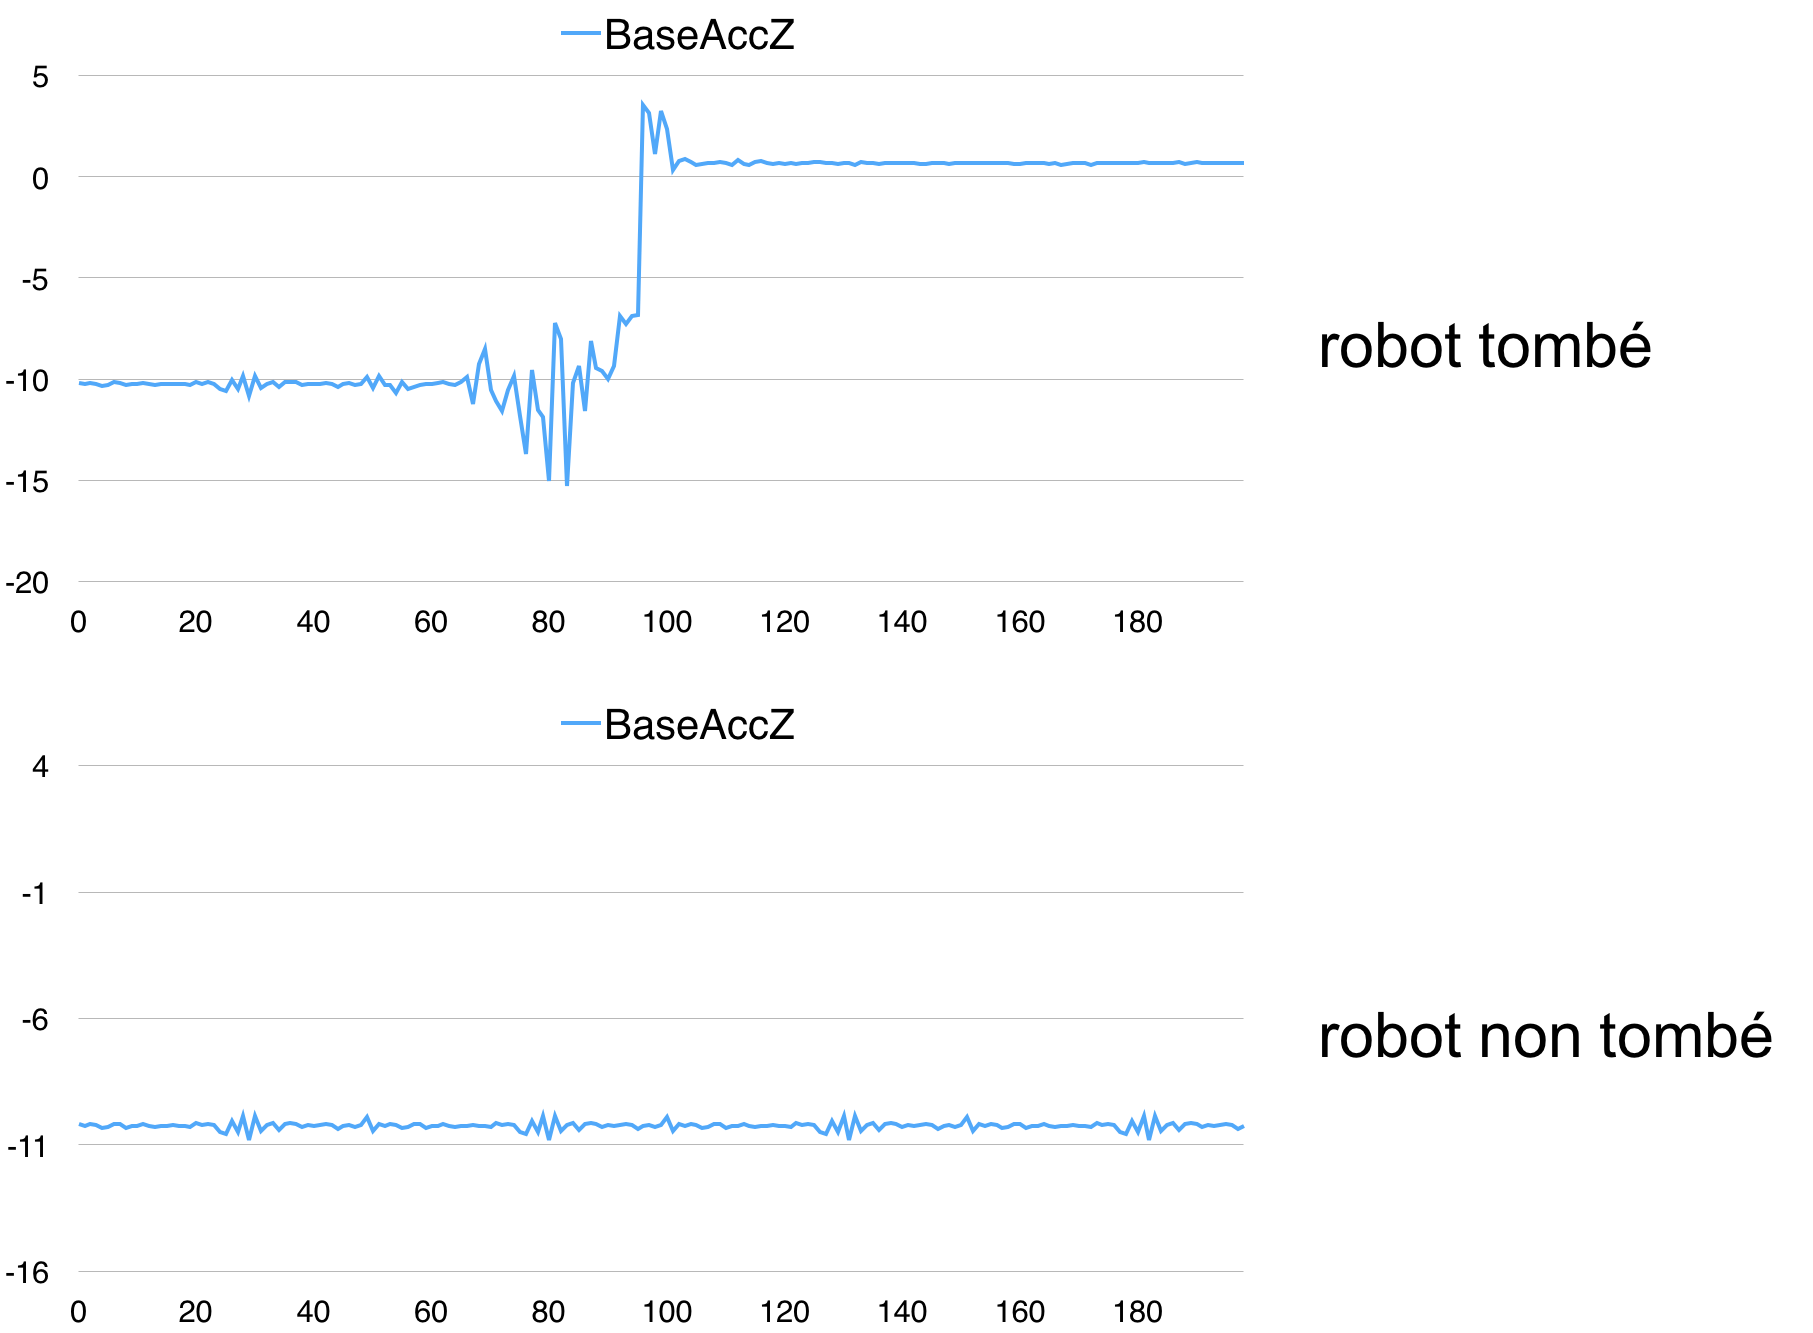
\includegraphics[width=12cm]{images/fall_not_fall.png}
	\caption[Formes caractéristiques de BaseAccZ en temps normal et en cas de chute]{Formes caractéristiques de BaseAccZ en temps normal et en cas de chute. On observe sur le graphe inférieur l'évolution de BaseAccZ lors d'un fonctionnement normal du robot. Sur le graphique supérieur, on observe l'évolution de BaseAccZ lorsque le robot chute. On remarque que celle-ci à la forme d'un échelon, centré sur l'instant où le robot tombe.}
	\label{fig:Formes caractéristiques de BaseAccZ en temps normal et en cas de chute}
\end{figure}

\begin{figure}[h]
	\centering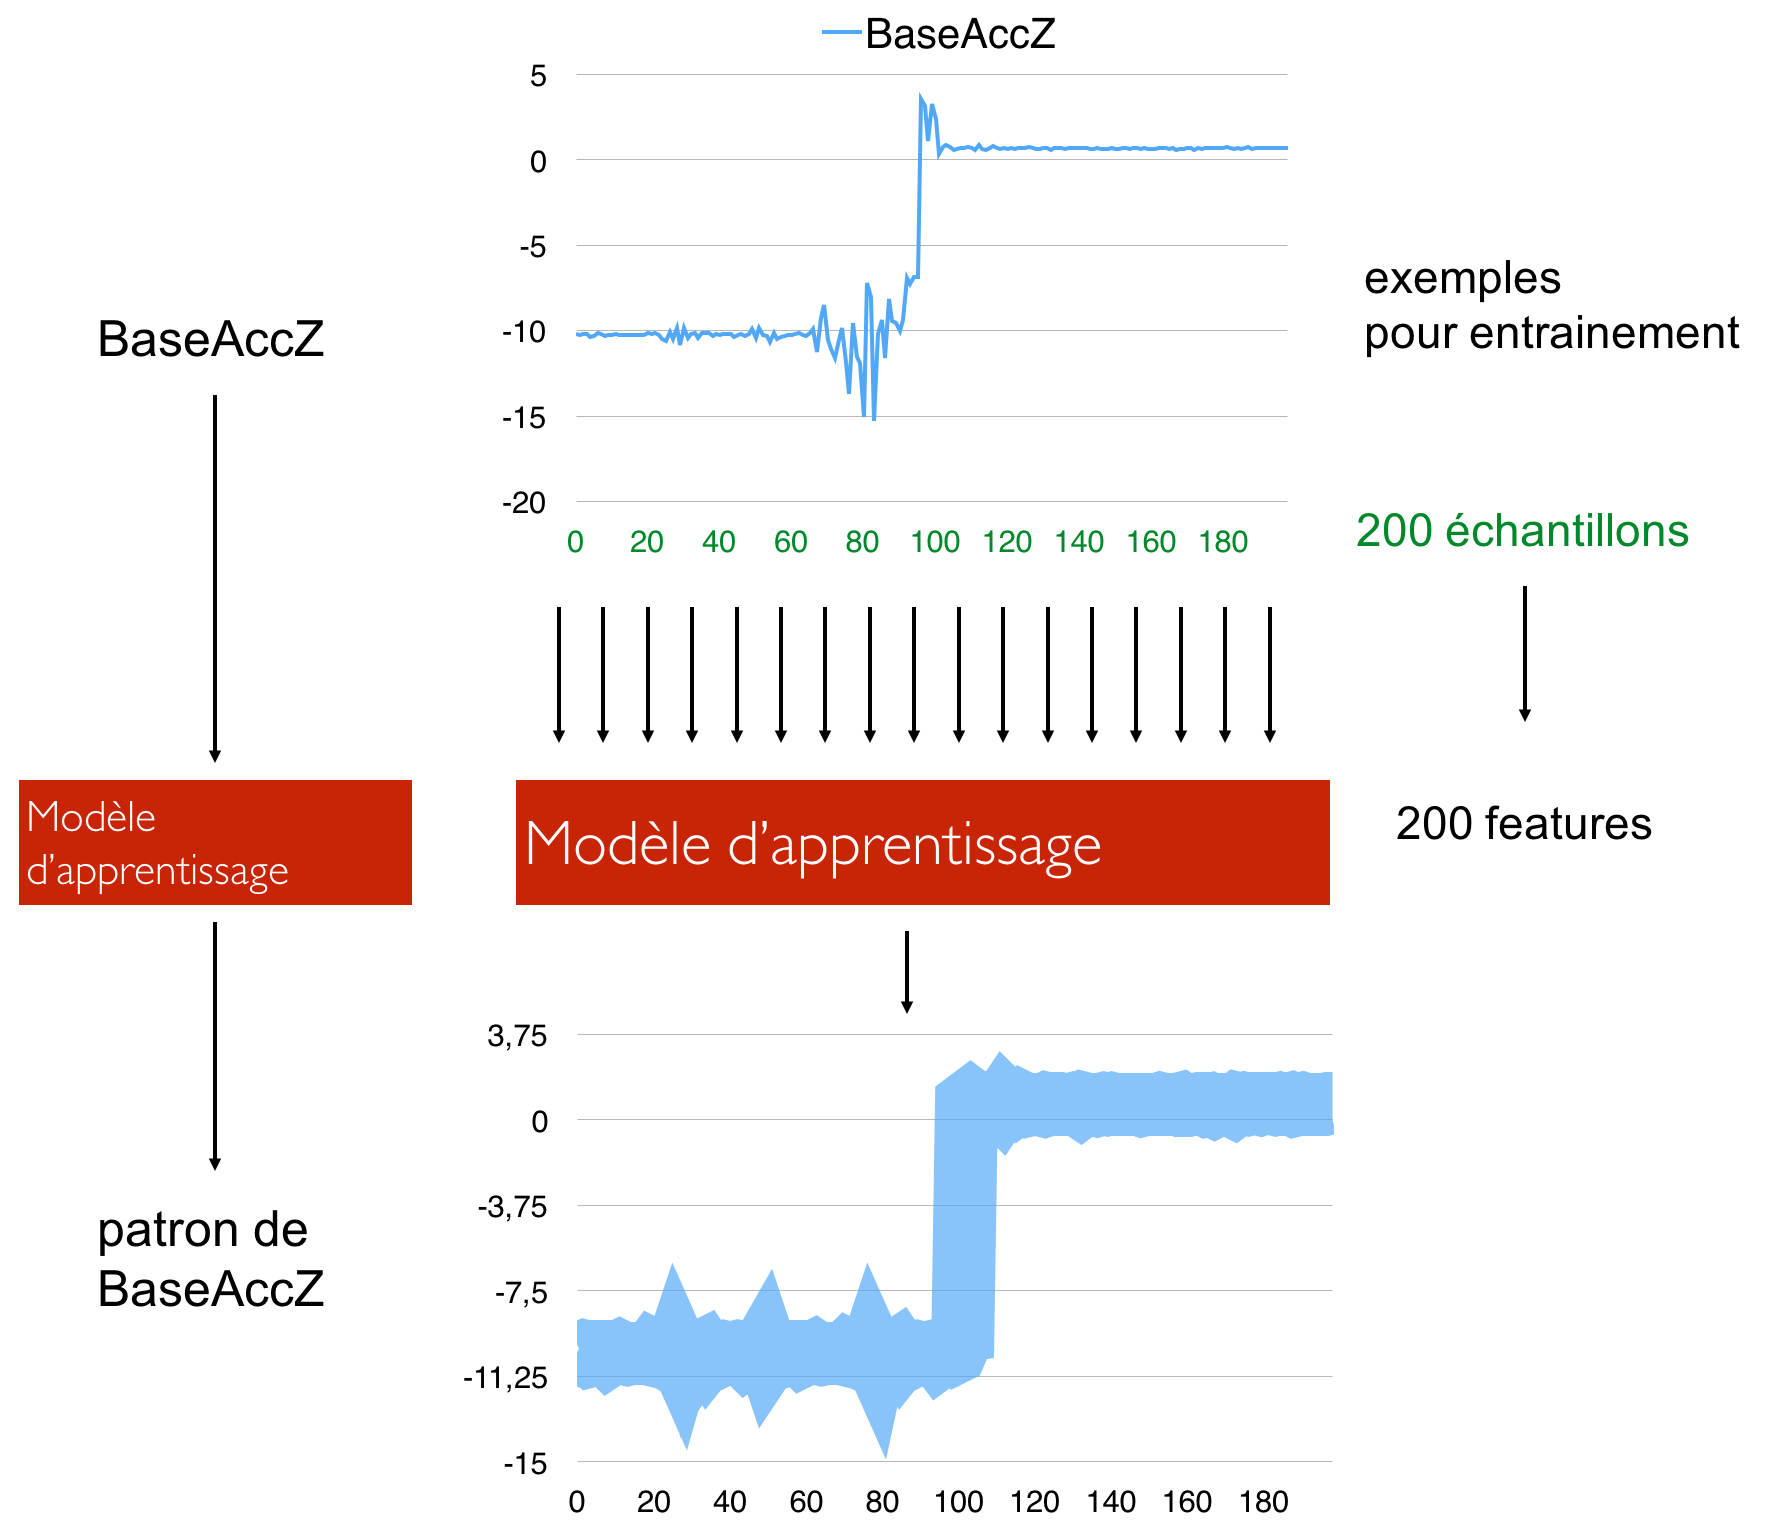
\includegraphics[width=12cm]{images/patron.png}
	\caption[Créer un patron caractéristique de la chute du robot]{Créer un patron caractéristique de la chute du robot. Chaque échantillon qui forment un exemple est considéré comme une entrée du système d'apprentissage, i.e. une feature. Entraîner l'algorithme à reconnaitre la forme de BaseAccZ, dans le case de robots tombés, revient à créer un patron de BaseAccZ qui caractérise la chute. L'entrainement s'effectue à partir de différents exemples de la feature BaseAccZ lorsque le robot tombe.}
	\label{fig:Créer un patron caractéristique de la chute du robot}
\end{figure}

\begin{figure}[h]
	\centering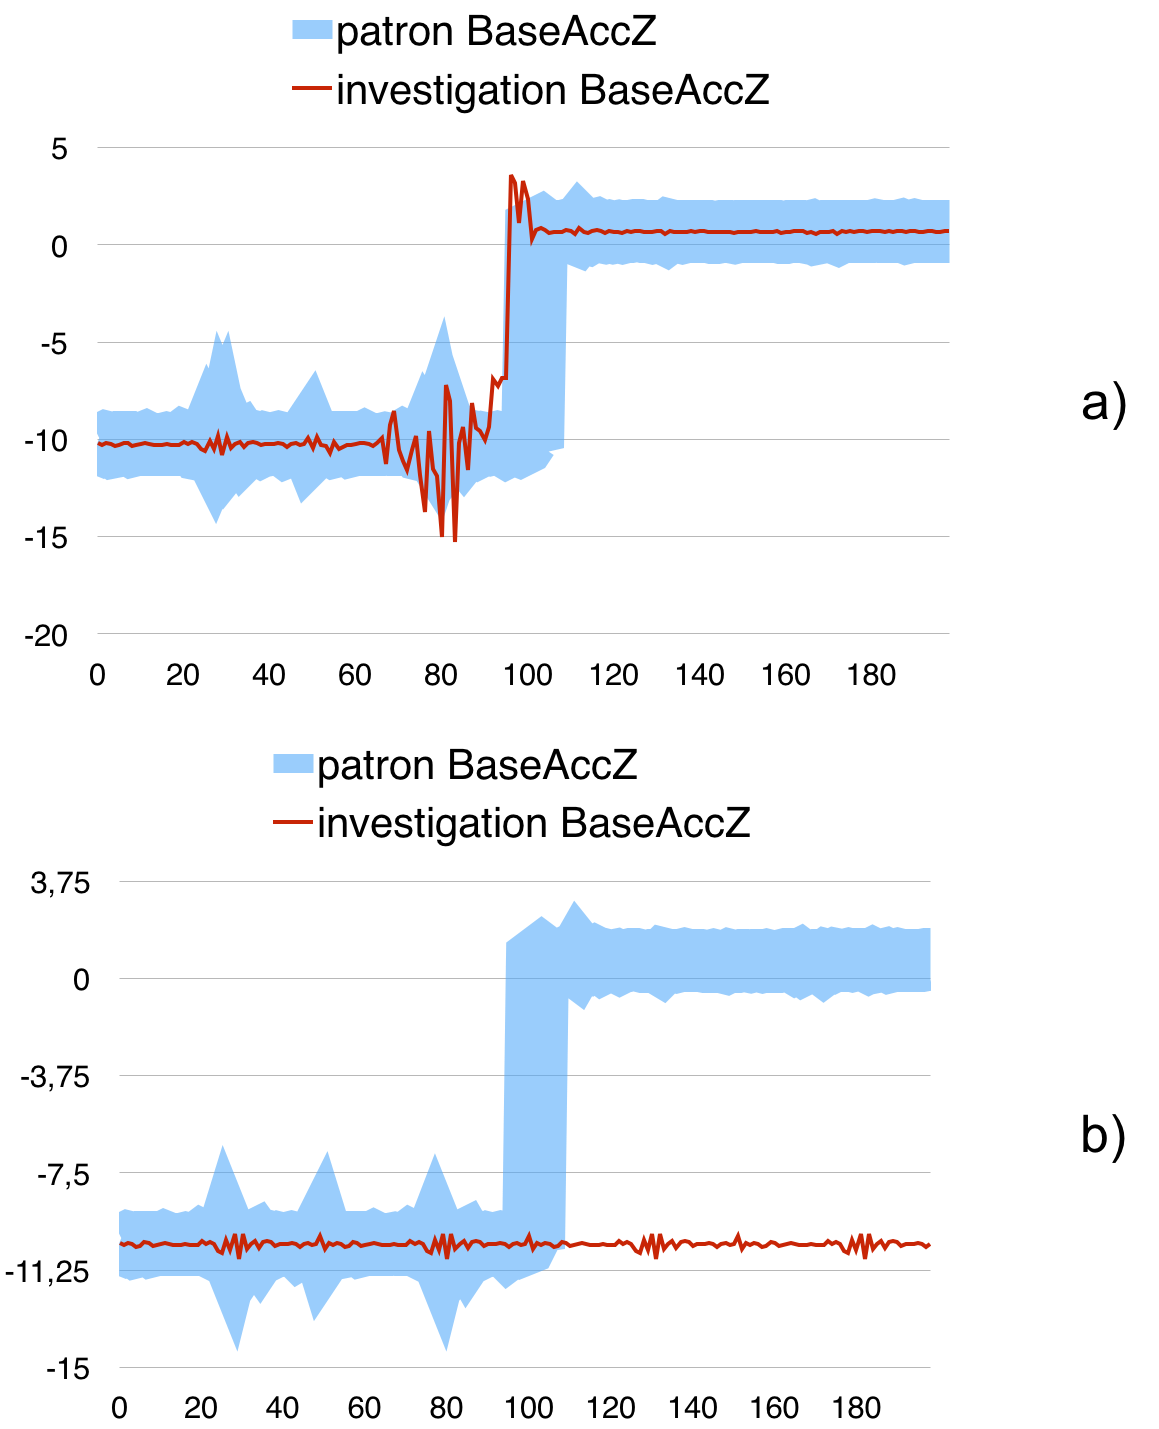
\includegraphics[width=12cm]{images/patron_comp.png}
	\caption[Détection d'une chute à partir du patron de BaseAccZ]{Détection d'une chute à partir du patron de BaseAccZ. Afin de savoir si l'exemple que l'on étudie est lié à une chute de robot ou non, on compare la valeur BaseAccZ du fichier log au patron caractéristique d'une chute de BaseAccZ. Sur le graphique supérieur, on observe que BaseAccZ est globalement contenu dans le patron, il s'agit donc d'un fichier log généré lors de la chute d'un robot. On observe en revanche sur le graphique inférieur que BaseAccZ n'est que \textbf{partiellement} incluse dans le patron. Il ne s'agit donc pas d'un exemple caractéristique d'une chute. }
	\label{fig:Détection d'une chute à partir du patron de BaseAccZ}
\end{figure}

Au vu des tests réalisés, cette méthode ne semble pas viable. En effet, comme on peut l'observer sur le graphique inférieur de la figure \ref{fig:Détection d'une chute à partir du patron de BaseAccZ}, même si la feature BaseAccZ n'est pas totalement inclue dans le patron, elle l'est \emph{partiellement} et ce sur pratiquement la moitié de son évolution. A cause de ce constat, l'algorithme considère dans certains cas un exemple comme caractéristique d'une chute alors qu'il ne l'est pas en réalité. Pour répondre à ce problème on propose que, plutôt que de créer un patron de la totalité de la courbe, on va seulement entraîner un algorithme à reconnaitre une certaine portion caractéristique de la courbe. Dans le cas de la détection d'une chute du robot, il s'agit du saut de valeur qui apparait sur la valeur de l'accélération en z du robot (BaseAccZ). On réalise de la reconnaissance de motifs. 

\subsection{Reconnaissance de motifs}
\label{Automatisation du processus d'investigation: Reconnaissance de motifs}
Au regard des études réalisées sur les différentes solutions qui s'offraient à nous pour la détection d'une root cause (cf. partie \ref{Automatisation du processus d'investigation: Reconnaissance de motifs: Différentes approches étudiées}), on souhaite à présent se tourner vers la reconnaissance de motif. 

\subsubsection{Principes généraux}
\label{Automatisation du processus d'investigation: Reconnaissance de motifs: Principes généraux}
D'une certaine manière, la reconnaissance de motif s'appuie sur une stratégie d'investigation proche de celle de l'Homme. On se place par exemple dans le cas où on souhaite déterminer la cause ayant entraîné la chute d'un robot. La cause correspond à la \emph{root cause} et la chute du robot à \emph{l'error name}. En tant qu'humain, on visualise et analyse les différentes courbes contenues dans le fichier log, généré lors de la détection de la chute au cours du Filtering Test. On observe alors les courbes de l'évolution de la position du senseur (clé HipPitchPositionSensorValue) et de l'actuateur (clé HipPitchPositionActuatorValue) de la hanche, figure \ref{fig:Évolution de la position du senseur et de l'actuateur de la hanche}. On remarque qu' à $t \approx 440 s$, le senseur se met à ne plus suivre la valeur de l'actuateur. L'étude réalisée partie \ref{Introduction:Expression du besoin:Exemple d'analyse d'une anomalie} nous \textbf{apprend} que cette particularité est la caractéristique d'un frottement des freins de la hanche. Ainsi, si on étudie ultérieurement un autre fichier log généré lors de la chute d'un robot et qu'on découvre ce motif, on en déduit aisément que le robot est également tombé à cause du frottement des freins de sa hanche. Plus on va observer de nouveaux cas, plus l'image que l'on a du motif caractéristique de cette \emph{root cause} va se préciser.\\
Dans le cadre du développement de notre algorithme, le principe est le même: on commence tout d'abord à apprendre la forme caractéristique de la root cause et une fois qu'on souhaite investiguer un nouveau fichier log, on compare ce motif caractéristique aux données du fichier. 

\begin{figure}[h]
	\centering\includegraphics[width=12cm]{images/HipPitch.png}
	\caption[Évolution de la position du senseur et de l'actuateur de la hanche]{Évolution de la position du senseur et de l'actuateur de la hanche.}
	\label{fig:Évolution de la position du senseur et de l'actuateur de la hanche}
\end{figure}

\paragraph{Apprentissage} La phase d'apprentissage s'appuie sur les principes évoqués en partie \ref{Automatisation du processus d'investigation: Reconnaissance de motifs: Différentes approches étudiées: Considérer chaque unité de temps comme une feature}. On considère que chaque échantillon (ou unité de temps) qui compose un exemple devient l'entrée de notre système d'apprentissage. A la différence qu'on considère qu'une partie de la courbe de nos exemples, le motif caractéristique. Par exemple, si on souhaite créer une nouvelle root cause "frottement des freins de la hanche", on sélectionnera sur chaque exemple le motif caractéristique de celle-ci (cf. figure \ref{fig:Créer un patron du motif caractéristique de la root cause "frottement des freins de la hanche"}). Le système d'apprentissage va donc uniquement apprendre le patron caractéristique du motif caractéristique et non de la courbe dans sa globalité. Les exemples devant être de la même taille on veille à sélectionner le même nombre d'échantillons pour chacun des motifs. On présente au système également des exemples ne contenant pas le motif, afin que l'algorithme bénéficie des deux types de labels pour son entrainement (root cause présente = 1, root cause non présente = 0).

\begin{figure}[h]
	\centering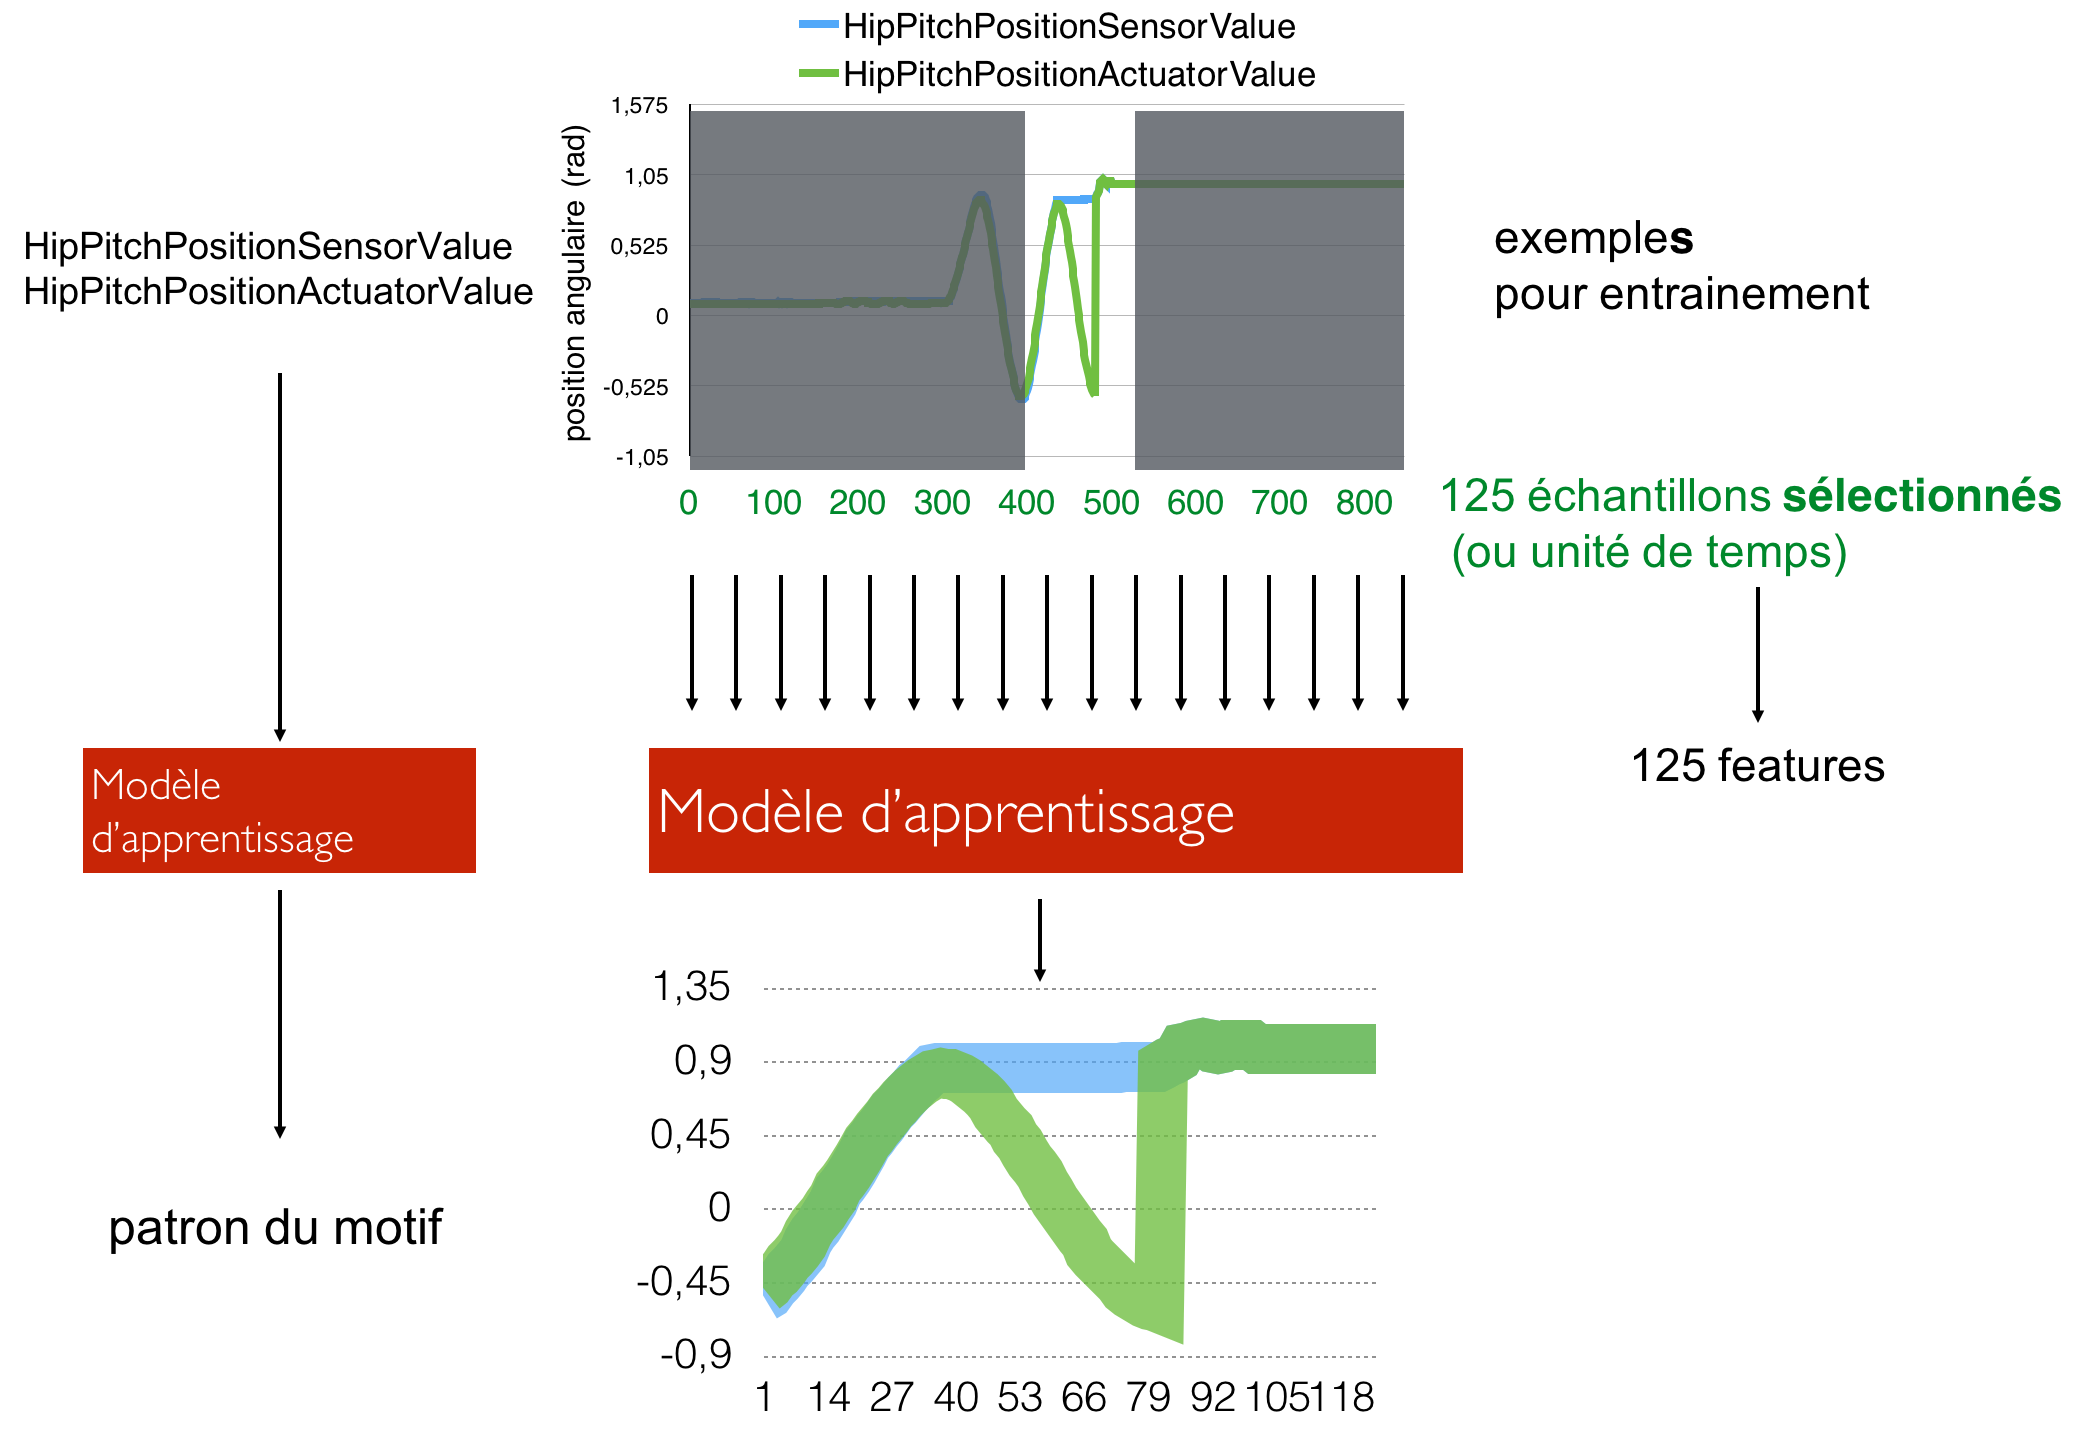
\includegraphics[width=14cm]{images/patron_motif.png}
	\caption[Créer un patron du motif caractéristique de la root cause "frottement des freins de la hanche"]{Créer un patron du motif caractéristique de la root cause "frottement des freins de la hanche". Chaque échantillon qui forment un motif est considéré comme une entrée du système d'apprentissage, i.e. une feature. Entraîner l'algorithme à reconnaitre le motif caractéristique formé par les courbes du HipPitchPositionSensorValue et HipPitchPositionActuatorValue revient à créer un patron caractéristique des deux features qui caractérise le frottement des freins de la hanche, dans le cadre de la chute robot. L'entrainement s'effectue à partir de différents exemples de motifs des deux features.}
	\label{fig:Créer un patron du motif caractéristique de la root cause "frottement des freins de la hanche"}
\end{figure}

\paragraph{Investigation}
Lorsque l'on souhaite investiguer un fichier pour déterminer la \emph{root cause} ayant entrainé l'apparition de l'\emph{error name} durant le Filering Test, on extrait la valeur des features du fichier log qui sont liées à la \emph{root cause}, puis on recherche le motif caractéristique. Pour cela, on découpe les courbes des features en plusieurs petits tronçons de la même taille que le motif caractéristique, et on les compare avec le motif caractéristique. Si ils sont globalement similaires au patron, on en déduit que la root cause a été détecté. Dans le cas contraire, on en déduit qu'elle n'a pas été détecté. En réalité, l'algorithme d'apprentissage automatique (SVM) nous retourne en sortie la probabilité avec laquelle le motif caractéristique a été détecté dans les courbes des features. On propose l'exemple d'investigation en figure \ref{fig:Balayage des features pour retrouver le motif caractéristique d'une root cause}).

\begin{figure}[h]
	\centering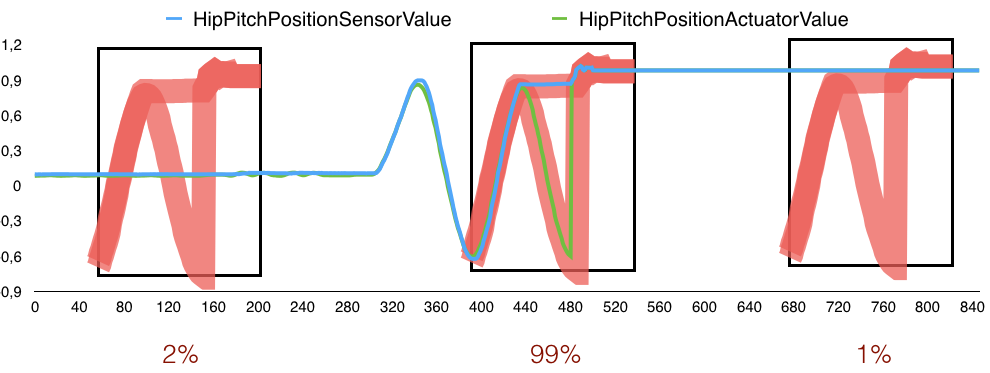
\includegraphics[width=12cm]{images/balayage_motif.png}
	\caption[Balayage des features pour retrouver le motif caractéristique d'une root cause]{Balayage des features pour retrouver le motif caractéristique d'une root cause. On observe que le premier et le dernier tronçon de la courbe des features HipPitchPositionSensorValue et  HipPitchPositionActuatorValue ne correspondent pas au motif caractéristique de la root cause "frottement des freins de la hanche". La probabilité en sortie du système est donc faible. Le deuxième tronçon correspond au motif caractéristique de la courbe, la probabilité en sortie du système est donc élevée.}
	\label{fig:Balayage des features pour retrouver le motif caractéristique d'une root cause}
\end{figure}

L'ensemble des probabilités en sortie des différents tronçons étudiés forment un courbe de probabilité. Si cette courbe dépasse un certain seuil, on considère la \emph{root cause} comme ayant été détectée. On propose la courbe de probabilité de la \emph{root cause} "frottement des freins de la hanche" en figure 	\ref{Automatisation du processus d'investigation}{fig:Courbe de probabilité de la root cause "frottement des freins de la hanche"}.

\begin{figure}[h]
	\centering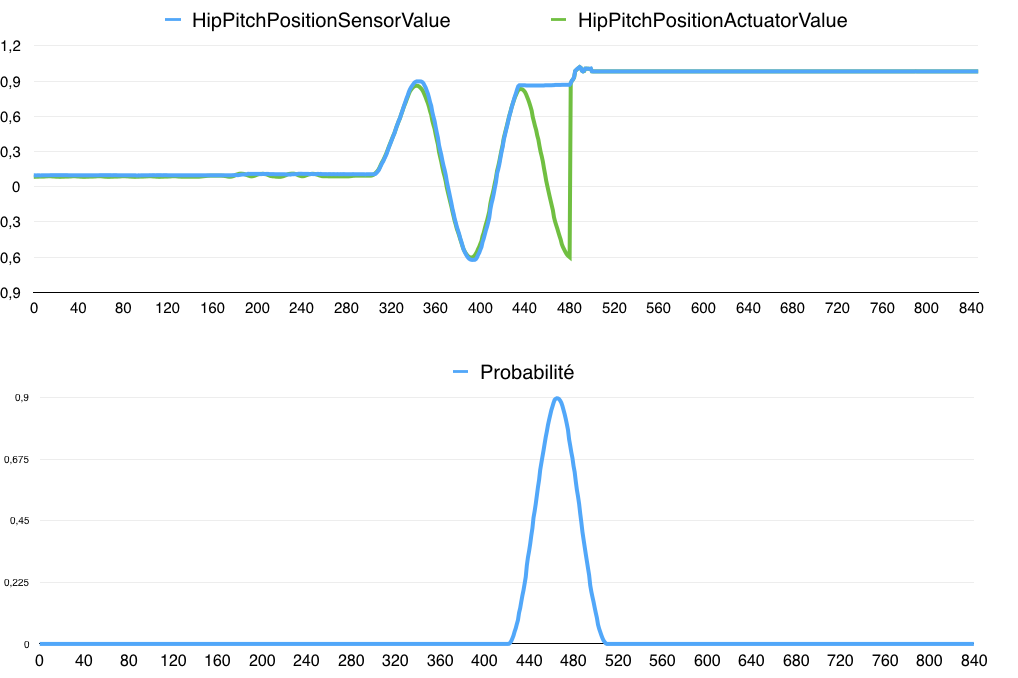
\includegraphics[width=12cm]{images/proba_motif.png}
	\caption[Courbe de probabilité de la root cause "frottement des freins de la hanche"]{Courbe de probabilité de la root cause "frottement des freins de la hanche".  On observe que lorsque l'on s'approche du motif caractéristique de la \emph{root cause}, la probabilité augmente fortement. Elle est au contraire faible sur les autres tronçons de la courbe.}
	\label{fig:Courbe de probabilité de la root cause "frottement des freins de la hanche"}
\end{figure}

\subsubsection{Exemples labellisés}
\label{Automatisation du processus d'investigation: Reconnaissance de motifs: Exemples labellisés}
Pour réaliser de l'apprentissage automatique, on rappelle que l'on a besoin d'exemples labellisés positifs (dans notre cas, le terme positif signifie des exemples de motifs caractéristiques de la \emph{root cause}) et des exemples labellisés négatifs (des exemples qui ne correspondent pas au motif caractéristique de la \emph{root cause}) . Ces exemples forment alors des classes. Dans le cadre de la \emph{root cause} "frottement des freins de la hanche", on peut visualiser l'ensemble de ces exemples et ces classes dans un repère construit à partir des features "position du senseur de la hanche" (clé HipPitchPositionSensorValue) et "position de l'actuateur de la hanche" (clé HipPitchPositionActuatorValue)


\subsubsection{Représentation des données}
\label{Automatisation du processus d'investigation: Reconnaissance de motifs: Représentation des données}


\subsubsection{Déroulement des données}
\label{Automatisation du processus d'investigation: Reconnaissance de motifs: Déroulement des données}







\section{Performances de la solution}
\label{Automatisation du processus d'investigation: Performances de la solution}
Une fois l'architecture du système définie, on souhaite mesurer les performances de l'algorithme.

\subsection{Optimisation des paramètres du SVM}
\label{Industrialisation du produit: Performances de la solution:Optimisation des paramètres du SVM}
La prise de décision de la part de l'algorithme du SVM peut être contrôlé via deux paramètres: C et gamma.
\begin{description}
	\item [gamma] 
	\item [C]
\end{description}

Afin de déterminer la meilleur combinaison de valeurs des deux paramètres, on calcule les \emph{courbes de validation}. Cela consiste à faire varier chacun des deux paramètres sur une plage de données et à calculer la précision de l'algorithme pour chaque valeur. On conserve la valeur optimale. 

\subsection{Matrices de confusion}
\label{Industrialisation du produit: Performances de la solution:Matrices de confusion}
Au début du processus, on sépare la base de données d'exemples en deux groupes : le \emph{training set} et \emph{test set}. Le premier jeu sert à entraîner l'algorithme SVM et l'autre permet d'en tester les performances. On rappelle que chaque exemple est labellisé, i.e. on connait  la sortie à laquelle ils sont corrélés (dans le cas de notre problématique, les labels étant \emph{root cause} présente ou non présente) 
\newline

Pour tester l'algorithme : 
\begin{enumerate}
	\item On commence par entrainer l'algorithme d'apprentissage automatique (SVM) à partir des exemples du \emph{training set}
	\item Une fois l'algorithme entraîné, on analyse chacun des exemples du \emph{test set}
	\item On compare ensuite la sortie prédite par l'algorithme et la sortie réelle (i.e. le label associé à chaque exemple). 
\end{enumerate}

Ainsi, on est capable de calculer le nombre de fois que l'algorithme a correctement prédit la sortie et lorsqu'il ne l'a pas fait. Ces résultats peuvent être exprimés sous la forme d'une matrice de confusion. Chaque colonne de la matrice représente le nombre d'occurrences d'une classe réelle (le label), tandis que chaque ligne représente le nombre d'occurrences de la classe prédite. Un des intérêts de la matrice de confusion est qu'elle montre rapidement si le système parvient à classifier correctement. 

\begin{table}[H]
	\centering
	\begin{tabular}{| c | c | c | c |}
		\hline
		\multicolumn{2}{|c|}{}  & \multicolumn{2}{|c|}{Classe réelle } \\
		\cline{3-4}
		\multicolumn{2}{|c|}{}  & Vrai & Faux \\
		\hline
		\multirow{2}*{Classe prédite} & Vrai & TP & FP \\
		\cline{2-4}
		& Faux & FN & TN \\
		\hline
	\end{tabular}
	\caption[Matrice de confusion]{Matrice de confusion}
	\label {tab:Matrice de confusion}
\end{table}

Avec : 
\begin{itemize}
	\item TP = True positive (en français vrai positif) correspond au nombre de résultats prédits positifs, là où ils étaient effectivement positifs.
	\item TN = True negative (en français vrai négatif) correspond au nombre de résultats prédits négatifs, là où ils étaient effectivement négatifs.
	\item FP = False positive (en français faux positif) correspond au nombre de résultats prédits positifs, là où ils étaient étaient en réalité négatifs.
	\item FN = False negative ( en français faux négatif) correspond au nombre de résultats prédits négatifs, là où ils étaient étaient en réalité positifs.
\end{itemize}
 
A partir de ces résultats, il est possible de déterminer la précision de l'algorithme:
\begin{equation}
	\text{accuracy}= \frac{TP + TN}{TP + TN + FP + FN}
	\label{accuracy}
\end{equation}
 
 \paragraph{Exemple}
 On soumet ici la matrice de confusion de la couche \emph{root cause} "frottement des freins de la hanche". 
 
\begin{table}[H]
	\centering
	\begin{tabular}{| c | c | c | c |}
		\hline
		\multicolumn{2}{|c|}{}  & \multicolumn{2}{|c|}{Classe réelle } \\
		\cline{3-4}
		\multicolumn{2}{|c|}{}  & Vrai & Faux \\
		\hline
		\multirow{2}*{Classe prédite} & Vrai & 45 & 0 \\
		\cline{2-4}
		& Faux & 0 & 15 \\
		\hline
	\end{tabular}
	\caption[Matrice de confusion]{Matrice de confusion}
	\label {tab:Matrice de confusion de la root cause "frottement des freins de la hanche"}
\end{table}

On observe qu'il n'y a aucun faux négatif et faux positif. Cela signifie que pour chaque exemple du \emph{test set}, l'algorithme à parfaitement prédit la sortie, i.e. qu'il a su à chaque fois détecter correctement si la root cause "frottement des freins de la hanche" était présente ou non dans le fichier log. D'après l'équation \ref{accuracy}, la précision de l'algorithme SVM de cette couche \emph{root cause} est donc de $100\%$.
 
\subsection{Courbes d'apprentissage}
\label{Industrialisation du produit: Performances de la solution:Courbes d'apprentissage}
Les courbes d'apprentissage représente la précision de l'algorithme d'apprentissage en fonction du nombre d'exemples utilisés pour l'entraînement du Machine Learning. 